\documentclass[conference]{IEEEtran}
%\documentclass[9pt]{sig-alternate}

\makeatletter
\newif\if@restonecol
\makeatother
\let\algorithm\relax
\let\endalgorithm\relax

\usepackage[ruled]{algorithm2e}
\usepackage{multirow}
%\usepackage[center]{caption}
\usepackage{setspace}
\usepackage{amsmath}
%\usepackage[pdftex]{graphicx}
%\usepackage{pdfpages}
\usepackage{multirow}
\usepackage{todonotes}
\usepackage{tikz}
\usepackage{xcolor}
\usepackage{pgfplots, pgfplotstable}
\usepackage{amsmath}
%\usepackage[ruled]{algorithm2e}
%\usepackage{multirow}
\usepackage{booktabs}
\usepackage{siunitx}
\sisetup{per=slash, load=abbr}

\usepackage{calc}
\usepackage{array}
\usepackage{caption}
\usepackage{subcaption}
\usepackage{rotating}


\usepackage{url}
\usepackage{pgf}
\usetikzlibrary{trees}
\usetikzlibrary{snakes,arrows,shapes}

%\usepackage{amsmath}
\usepackage{mdwlist}
%\usepackage[normal]{subfigure}
%\usepackage{subfig}

\usepackage{textcomp}


\usepackage{graphicx}
\usepackage{epstopdf}
\usepackage{epsfig}
\usepackage{listings}
\usepackage{xcolor}
\usepackage{dot2texi}
\usepackage{graphicx,stfloats}

\usepackage{graphicx,epstopdf}
\epstopdfsetup{update}

%\usepackage{listings}% http://ctan.org/pkg/listings
%\usepackage{subfig}% http://ctan.org/pkg/subfig
%\usepackage{lipsum}% http://ctan.org/pkg/lipsum

%\usepackage{enumitem}
\usepackage{enumerate}

%\subfigcapmargin = 3cm


\pgfplotsset{compat=newest}

\setlength{\paperheight}{11in}
\setlength{\paperwidth}{8.5in}


%\lstset { %
%	language=C,
%	backgroundcolor=\color{black!5}, % set backgroundcolor
%	%basicstyle=\footnotesize,% basic font setting
%	basicstyle=\ttfamily\tiny,
%	%\basicstyle=\ttfamily\scriptsize,
%	keywordstyle=\color{blue}\ttfamily,
%	stringstyle=\color{red}\ttfamily,
%	commentstyle=\color{green}\ttfamily,
%	breaklines=true
%}

% correct bad hyphenation here
\hyphenation{op-tical net-works semi-conduc-tor}
\newcommand*{\blind}{}

\begin{document}\sloppy
% paper title
% can use linebreaks \\ within to get better formatting as desired
%\title{An Area-Efficient Time-multiplexed FPGA Overlay Architecture using DSP Block based Functional Units}
\title{A Time-Multiplexed FPGA Overlay\\ with Linear Interconnect}
%\title{Architecture Exploration for the Linear Time-multiplexed FPGA Overlay}

\author{
	\IEEEauthorblockN{Xiangwei Li\IEEEauthorrefmark{1},
		Abhishek Kumar Jain\IEEEauthorrefmark{2},
		Douglas L. Maskell\IEEEauthorrefmark{1} and
		Suhaib A. Fahmy\IEEEauthorrefmark{3}}
	
	\IEEEauthorblockA{\IEEEauthorrefmark{1}School of Computer Science and Engineering, Nanyang Technological University, Singapore}
	\IEEEauthorblockA{\IEEEauthorrefmark{2}Lawrence Livermore National Laboratory, United States}
	\IEEEauthorblockA{\IEEEauthorrefmark{3}School of Engineering, University of Warwick, United Kingdom}
	\IEEEauthorrefmark{1}\{xli045, asdouglas\}@ntu.edu.sg
	\IEEEauthorrefmark{2}jain7@llnl.gov
	\IEEEauthorrefmark{3}s.fahmy@warwick.ac.uk}


%\author{\IEEEauthorblockN{Xiangwei Li}
%	\IEEEauthorblockA{SCSE\\
%		NTU Singapore\\
%		xli045@e.ntu.edu.sg}
%	\and
%	\IEEEauthorblockN{Abhishek Kumar Jain}
%	\IEEEauthorblockA{Lawrence Livermore \\ National Lab., USA\\
%		jain7@llnl.gov}
%	\and
%	\IEEEauthorblockN{Douglas L. Maskell}
%	\IEEEauthorblockA{SCSE\\
%		NTU Singapore\\
%		asdouglas@ntu.edu.sg}
%	\and
%	\IEEEauthorblockN{Suhaib A. Fahmy}
%	\IEEEauthorblockA{School of Engineering\\
%		University of Warwick, UK\\
%		s.fahmy@warwick.ac.uk}}

% make the title area
\maketitle
%\setlength{\baselineskip}{10.3pt}

\begin{abstract}
Coarse-grained overlays improve FPGA design productivity by providing fast compilation and software like programmability. Soft processor based overlays with well-defined ISAs are attractive to application developers due to their ease of use. However, these overlays have significant FPGA resource overheads. Time multiplexed (TM) CGRA-like overlays represent an interesting alternative as they are able to change their behavior on a cycle by cycle basis while the compute kernel executes. This reduces the FPGA resource needed, but at the cost of a higher initiation interval (II) and hence reduced throughput.

%Current CGRA-like overlays have a high resource overhead due to the implementation of a fully flexible routing network. However, many application kernels are acyclic and can be implemented using a much simpler linear feed-forward routing network. 
The fully flexible routing network of current CGRA-like overlays results in high FPGA resource usage. However, many application kernels are acyclic and can be implemented using a much simpler linear feed-forward routing network. This paper examines a DSP block based TM overlay with linear interconnect where the overlay architecture takes account of the application kernels' characteristics and the underlying FPGA architecture, so as to minimize the II and the FPGA resource usage. We examine a number of architectural extensions to the DSP block based functional unit to improve the II, throughput and latency. 
The results show an average 70\% reduction in II, with corresponding improvements in throughput and latency. 

\begin{comment}
The proposed overlays are relatively efficient consuming just 5-8\% of the Zync resources while operating at close to the maximum DSP frequency. Application kernels mapped to the overlay result in an average 70\% reduction in II compared to the overlay in~\cite{li2016area}, with improvements in throughput and latency.

\end{comment}

%Coarse grained FPGA overlay architectures have emerged as an attractive solution for improving accelerator design productivity by offering fast compilation and software-like programmability. Throughput oriented spatially-configurable FPGA overlays can deliver maximum performance at the cost of significant resource requirement due to the use of one functional unit for each compute kernel operation. Alternatively, time-multiplexing the FU within an overlay architecture can significantly reduce the FU and interconnect resource requirements but at the cost of a higher initiation interval (II). Such a time-multiplexed overlay with its reduced FPGA resource requirements can be thought of as a rapidly reconfigurable data-flow accelerator within a large accelerator framework allowing the remainder of the FPGA fabric to be utilized for other purposes. However, the exact architecture of such a time-multiplexed overlay needs to be carefully designed taking into account the characteristics of the application kernels and the underlying FPGA architecture, so as to minimize the II and FPGA resource usage for improving the throughput per unit area. This paper examines the possibility of minimizing the II while adding minimal resources in the overlay FU so that throughput per unit area can be improved. We demonstrate significant reduction in II by using architectural optimizations such as the use of rotating register files which allows overlapping of data communication and computation. We also propose replication of the execution datapath while sharing the fetch/decode/control hardware and instruction memory to improve the compute density of the FU. The results presented show a quadruple reduction in II while only doubling the FPGA resource consumption resulting in improved throughput per unit area.


\end{abstract}

\begin{IEEEkeywords}
Reconfigurable system, overlay architecture, FPGA
%field programmable gate arrays.
\end{IEEEkeywords}


%\IEEEpeerreviewmaketitle

\pagenumbering{arabic}
%!TEX root=../draft.tex
%\vspace{-6pt}
\section{Introduction}
\label{ch1_introduction}

There has been a resurgence in FPGA-based accelerators due to developments in the cloud computing and IoT domains. 
FPGA accelerators are often custom designed to achieve maximum performance, using conventional RTL hardware design techniques, and as such, are only applied to specific algorithms in specific applications, and hence are fixed, negating many of the benefits of the programmable FPGA device. This design process is long and complex, requiring low-level device expertise and special knowledge of both hardware and software systems, resulting in major design productivity issues and long compilation times, which limit the mainstream adoption of FPGA based accelerators for general purpose computing. 
%for general purpose computing~\cite{stitt2011field}.

High-level synthesis (HLS) has been widely adopted by EDA tool vendors to address the design productivity issue. However, to maximize performance, detailed low-level design effort is often still required, making design difficult for non-experts. Additionally, while HLS tools have allowed designers to focus on high-level functionality instead of low-level details, the back-end flow (specifically the FPGA place and route) requires very long compilation times, particularly for large designs, contributing to the lack of productivity and mainstream adoption of FPGAs. In many cases, the time required to change an FPGA configuration limits hardware accelerators to predesigned static (i.e. fixed) implementations, negating the fundamental benefit of FPGAs. To be more appealing to the broader group of application developers, who are used to software API abstractions and fast development cycles, the FPGA hardware resource needs to be better abstracted.

One possible solution to this problem is to use an overlay (a programmable coarse-grained hardware abstraction layer on top of the FPGA fabric) as this simplifies both the hardware design and mapping process. This then allows the FPGA to be treated as a virtualized execution platform that both abstracts the hardware details and enables runtime management support, so that the hardware can be viewed as just another software-managed task, possibly even controlled by the OS or a hypervisor~\cite{jain2014virtualized}. This results in better application management, and has the potential for allowing portability across devices, software-like programmability by mapping from high-level descriptions, better design reuse, fast compilation by avoiding the complex FPGA design flow (particularly the very slow place and route process), resulting in improved design productivity. Another significant advantage is rapid application swapping (a hardware context switch) as coarse-grained overlay architectures have smaller configuration data sizes than fine-grained FPGAs.  The major problem is that many of the current overlays are not efficient (in area, power, throughput, etc.) and still require FPGA-like configuration times, as in many cases the overlay needs to change when the application requiring acceleration needs to change.

%!TEX root=../draft.tex
%\vspace{-6pt}
\section{Related Work}
\label{ch2_related_work}

%A number of approaches have been developed to implement TMFU-TMN Overlays, ranging from simple processors to highly configurable logic arrays.
%In a nutshell, these overlays can be implemented as soft processors~\cite{cheah2014idea,laforest2012octavo,gray2016grvi}, vector processors~\cite{severance2013embedded}, coarse-grained reconfigurable arrays~\cite{brant2013coarse,paul2012remorph,liu2013soft,rashid2014comparing}, and GPU-like overlays~\cite{al2016fgpu}.

Overlays come in many forms, with the most common being spatially configured~\cite{jain2016deco, coole2010intermediate} and time multiplexed (TM)~\cite{severance2013embedded, liu2013soft}. 
Spatially configured overlays fully unroll the kernel onto a pipelined array of FUs, resulting in an initiation interval (II) of 1.
They provide high performance, but require significant FPGA resources. 
TM overlays change their behavior on a cycle by cycle basis, thus reducing the amount of FPGA resource dedicated to the functional unit (FU) and interconnect, but at the cost of a higher II and hence a reduced throughput. 

%The most successful TM overlays are based on soft processors.
%, such as CPUs~\cite{laforest2012octavo, nios2009processor}, vector processors~\cite{severance2013embedded} and GPU-like architectures~\cite{al2016fgpu}. 
%The most successful TM overlays are based on soft processors, such as CPUs~\cite{laforest2012octavo, nios2009processor, al2012guppy}, vector processors~\cite{severance2013embedded} and GPU-like architectures~\cite{al2016fgpu}. Guppy is GPU-like??? Anyway delete it. Have enough.
%But they are normally conventional processing elements.
%Examples of some of the more performance oriented soft processor solutions include:
Most successful TM overlays are based on soft processors. 
The more performance oriented ones include, SIMD Octavo~\cite{laforest2017microarchitectural}, VectorBlox MXP~\cite{severance2013embedded} and VLIW TILT~\cite{Ovtcharov2013TILT}. A massively parallel overlay, called GRVI Phalanx~\cite{gray2016grvi}, based on the RISC-V processor and the Hoplite NOC~\cite{kapre2015hoplite} mapped 1680 RISC-V cores onto an UltraScale+ VU9P.
These overlays have the advantage of a well-known, well-designed ISA which makes them easy to use, however, they utilize a large amount of FPGA resource and have a significant power consumption.

\begin{comment}
%Octavo
The Octavo soft processor~\cite{laforest2012octavo}, which is a multi-threaded 10-stage pipelined architecture designed to operate at the maximum frequency of the Block RAMs (550MHz) on a Stratix IV FPGA. 
The Octavo was further extended to support SIMD by duplicating the datapath with a shared instruction stream~\cite{laforest2017microarchitectural}. 
VectorBlox MXP~\cite{severance2013embedded} is a soft vector processor with fracturable ALUs that can support 8-bit to 32-bit fixed-point operations. 
Increasing the number of vector lanes in MXP results in very high FPGA resource utilization and significant clock frequency degradation.
SIMD-Octavo was compared with VectorBlox MXP~\cite{severance2013embedded} and operates at about double the clock frequency of MXP and generally achieves better performance (for an equal number of lanes), in terms of execution time, area and area-delay product. The execution time of multi-lane SIMD-Octavo is better than hand-crafted Verilog HDL, but requires one to two orders of magnitude more hardware resource. 
%overlay with 32 lanes achieves up to 8.7$\times$ speedup on throughput within 32 lanes, it suffers up to 319$\times$ area overhead.

%TILT
TILT~\cite{Ovtcharov2013TILT} is a VLIW soft processor with deeply-pipelined floating-point FUs targeting Stratix IV FPGAs.
An 8-core TILT system consumed approximately 12K eALMs, fractionally more than Octavo and slightly less than MXP, while operating at just above 200MHz (about the same as MXP).
TILT~\cite{rashid2014comparing} achieved about half the compute density of implementations mapped directly to the FPGA using OpenCL HLS.


%GRVI Phalanx
GRVI Phalanx~\cite{gray2016grvi} is a massively parallel overlay based on an FPGA-efficient implementation of the RISC-V soft processor. The GRVI processor uses just 320 LUTs and runs at a frequency of up to 375MHz on a Kintex UltraScale FPGA. Multiple GRVI processors with shared memory and local interconnect, are formed as clusters, which efficiently communicate with each other via a Hoplite NOC~\cite{kapre2015hoplite}. Implementations with 400 and 1680 RISC-V cores on a Kintex UltraScale KU040 and a Virtex UltraScale+ VU9P have been reported. Currently there is minimum tool support for this platform with no application performance comparisons with other overlays. 


%MXP
%VectorBlox MXP~\cite{severance2013embedded} is a soft vector processor with fracturable ALUs that can support 8-bit to 32-bit fixed-point operations. 
%Increasing the number of vector lanes in MXP results in very high FPGA resource utilization and significant clock frequency degradation.
%
%MXP can operate at over 200 MHz on a Stratix IV device with less than 16 vector lanes. 
%%A 64-lane configuration demonstrated up to 918$\times$ speedup in comparison with Nios II processor on matrix multiplication.
%However, the scalability of SVPs is limited by the number of vector lanes (A maximum of 32-lane vector engine can be mapped on Cyclone IV-115). 
%While increasing the number of vector lanes introduces intensive resource consumption, it also leads to clock frequency degradation.

%FGPU (not a performance overlay, so removed).
%FGPU~\cite{al2016fgpu} is a soft GPU-like overlay ???  was proposed as a flexible solution for software tasks.
%It achieves up to 48.5$\times$ speedup over the MicroBlaze on ZC706 FPGA board, at the penalty of 17.7$\times$ area overhead.
%However, the FGPU is designed with a massive pipeline of 18 stages to fulfill the high performance.
%Due to the intensive complexity of the compute units, even the FGPU with only 8 CUs consumes 124K LUTs on z7045 Zynq, which corresponds to 57\% of the available resource.
\end{comment}

An alternative solution is to build arrays of customized TM FUs and interconnect on the FPGA, similar to CGRAs~\cite{mei2003adres}. 
%They are generally highly pipelined ALUs/PEs, along with an array based interconnect. 
%I do not think this is necessary%%The CGRA-like overlays have been proved to be a suitable solution for compute intensive loop acceleration~\cite{liu2015quickdough}.
A number of different interconnect styles for connecting between FUs can be used, with the most common being: island style~\cite{coole2010intermediate, jain2015efficient}, nearest neighbor~\cite{paul2012remorph, liu2013soft} and to a lesser extent linear interconnect~\cite{capalija2011towards, jain2016deco}.
%or having no interconnection~\cite{rashid2014comparing}.
The overhead of the interconnect network, particularly for island style and nearest neighbor interconnects, contribute to a significant FPGA resource utilization.
%caused by the flexible routing network still remains a problem to be solved~\cite{coole2010intermediate}. 
Examples of CGRA-like TM overlays include:



%CARBON
CARBON~\cite{brant2013coarse}, a CGRA-like overlay implemented as a 2$\times$2 array of tiles on a Stratix III FPGA. Each CARBON tile has an FU with a programmable ALU and instruction memory, supporting up to 256 instructions. 
%An FU consumed 3K ALMs, 304 FFs, 15.6K BRAM bits and 4 DSP blocks, achieving a modest 90 MHz operating frequency.
CARBON has a large FU resource requirement with a relatively slow speed which limits its scalability, compared to the overlays discussed below.


%SCGRA
The SCGRA overlay~\cite{liu2013soft} was proposed to address FPGA design productivity issues. 
Application specific SCGRA overlays were implemented on Zynq~\cite{liu2015quickdough}, achieving a speedup of up to 9$\times$ compared to the same application running on the Zynq ARM processor. 
The 250 MHz FU consists of an ALU, multiport data memory (256$\times$32 bits) and customizable depth instruction ROM (Supporting 72-bit instructions) resulting in significant BRAM utilization. 
Fast application context switching is not possible as the full FPGA bitstream needs to be reconfigured for a compute kernel change.


%reMORPH
The reMORPH overlay~\cite{paul2012remorph} better targets the FPGA fabric, with an FU consuming 1 DSP Block, 3 block RAMs, 196 LUTs and 41 registers.
To reduce overhead, the reMORPH FU does not use decoders resulting in a 72-bit instruction memory (supporting up to 512 instructions) which also over utilizes the BRAMs.
reMORPH uses a nearest neighbor style of non-programmable interconnect, which is adapted using partial reconfiguration at runtime, and hence, suffers from the same slow hardware context switch problem as SCGRA.


Many TM overlays have large area overheads due to the routing resources, or large instruction storage requirements.
%, which along with their use of partial reconfiguration results in a long kernel context switch time. 
To address these problems, we propose a streaming architecture based on feed-forward pipelined datapaths, as streaming based accelerators have been highly successful when implemented in FPGAs~\cite{oliver2005reconfigurable, saqib2015pipelined}. Targeting highly compute intensive algorithms with little control and relatively simple dependencies allows us to use a linear interconnect structure, where data flows in a single direction from one FU to the next, thus minimizing the interconnect requirements. This structure then enables the use of a very simple and efficient streaming memory interface. The instruction storage is also reduced, as the architecture allows us to store just those instructions used by an individual FU. The reduced instruction and control requirements means that a lightweight processor architecture can be used, similar to the DSP based iDEA processor~\cite{cheah2014idea}, further reducing the hardware resource requirements while achieving a relatively high operating frequency.

\begin{comment}
Most of the time multiplexed overlays described above suffer from large area overheads due to the routing resources, or the large instruction storage requirements.
%, which along with their use of partial reconfiguration results in a long kernel context switch time. 
To address these issues, we propose a streaming architecture based on feed-forward pipelined datapaths, as accelerators based on the streaming model have been highly successful when implemented in FPGAs~\cite{oliver2005reconfigurable, saqib2015pipelined}. Targeting highly compute intensive algorithms with little control and relatively simple dependencies allows us to use a simple linear interconnect structure, where data flows in a single direction from one FU to the next, thus minimizing the interconnect requirements. This structure then enables the use of a very simple and efficient streaming memory interface. The instruction storage is also reduced, as the architecture allows us to store just those instructions used by an individual FU. The reduced instruction and control requirements means that a lightweight processor architecture can be used, similar to the DSP based iDEA processor~\cite{cheah2014idea}, further reducing the hardware resource requirements while achieving a relatively high operating frequency.
\end{comment}

% possibly include contributions in bullet form
% possibly mention organisation

%!TEX root=../draft.tex
%\vspace{-6pt}
\section{Linear TM Overlay}
\label{ch3_arch}

%\subsection{Data Streaming Model}
While overlays with a general-purpose mesh-based interconnect allow for flexible communication between each FU, they introduce a significant resource overhead associated with the routing network. 
In many cases, a simple linear interconnect structure can be used instead. In a TM overlay, this reduces the highly flexible interconnect to a direct connection between FUs, as in Fig.~\ref{pipelines}, and allows data flow graph (DFG) nodes from the same scheduling time step to be allocated to individual FUs~\cite{li2016area}.
The linear overlay consists of a streaming data interface made up of Distributed RAM (DRAM) acting as a FIFO, which feeds the cascade of time-multiplexed FUs, with another DRAM-based FIFO at the output.
Tasks are scheduled to the overlay using ASAP scheduling, with nodes at the same (horizontal) level allocated to a single FU.
For example, Fig.~\ref{code} shows the medical imaging `gradient' benchmark~\cite{cong2014fully}, while Fig.~\ref{dfg} shows the resulting DFG.
This example requires 4 FU stages, where the first stage contains 4 subtract operations which would execute on the first FU, then the 4 multiplication operations execute on the second FU, and so on.


\begin{figure}[b]
	\centering
	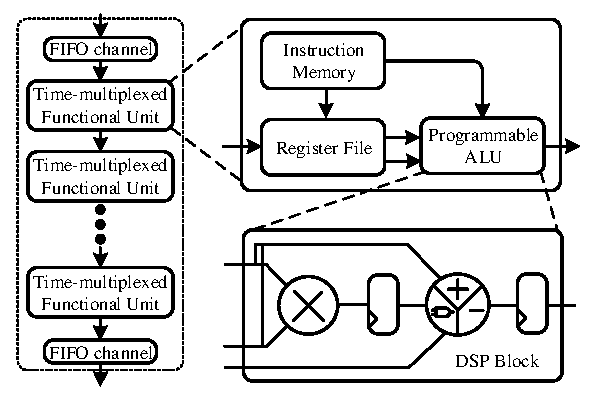
\includegraphics[width=7.5cm]{figures/pipelines_new.pdf}
	\caption{A linear TM overlay.}
	\label{pipelines}
\end{figure}

\begin{figure}[t]
	\centering
	\begin{subfigure}[t]{0.2\textwidth}
		\centering
		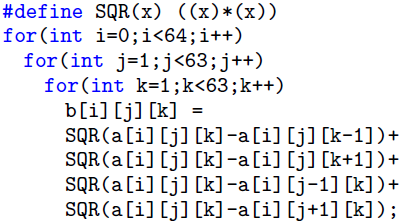
\includegraphics[width=4.6cm]{figures/code.png}
		\caption{C Source Code}
		\label{code}
	\end{subfigure}
	~~
	\begin{subfigure}[t]{0.24\textwidth}
		\centering
		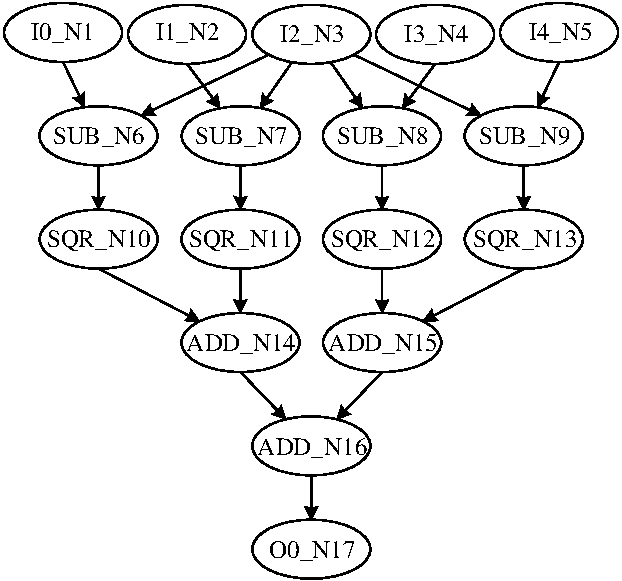
\includegraphics[width=4cm]{figures/DFG.pdf}
		\caption{Data Flow Graph}
		\label{dfg}
	\end{subfigure}
	\caption{The `gradient' benchmark.}
	\label{dfgs}
\end{figure} 


The FU uses the same principle as the iDEA DSP-based processor~\cite{cheah2012idea}, and requires 1 DSP block, 160 LUTs and 293 FFs and runs at 325 MHz on a Xilinx Zynq XC7Z020.
%Xilinx Zynq XC7Z020-1CLG484C.
The FU consists of a LUTRAM-based instruction memory (IM) and register file (RF), and a DSP-based ALU, as shown in Fig.~\ref{fu} (excluding all of the logic in the four dashed boxes). 
%Details of the microarchitecture can be found in~\cite{li2016area}. 

The major advantage of TM overlays is that an application kernel can be mapped to fewer FUs, reducing resource consumption at the expense of II. The example of Fig.~\ref{dfg} can be mapped onto a linear overlay with 4 FUs using ASAP scheduling and has an II of 11, consisting of 5 cycles for data entry, 4 cycles for the 4 subtract operations, 1 cycle for data output and 1 cycle to flush the pipeline.
%For the example shown in Fig.~\ref{dfg} the II is 11, consisting of 5 cycles for data entry, 4 cycles for the 4 subtract operations, 1 cycle for data output and 1 cycle to flush the pipeline.
%%Note that multiplexing the kernel operations of the DFG in Fig. 1(b) to a single FU would result in an II of 17 (5 load, 11 operation, and 1 store), assuming best case execution without NOP insertions, 
By comparison, a spatially configured overlay would have an II of 1, requiring 11 FUs.
However, using ASAP-based scheduling means that the overlay has a depth equal to the critical path of the DFG, and must be re-sized for each new application kernel, thus limiting its usefulness. 
Whereas,  a small linear overlay with a fixed depth that is able to map larger more general purpose compute kernels would be much more useful.
In the next sections, we examine mechanisms to increase the throughput and usability.


\begin{figure*}[!tb]
	\centering
	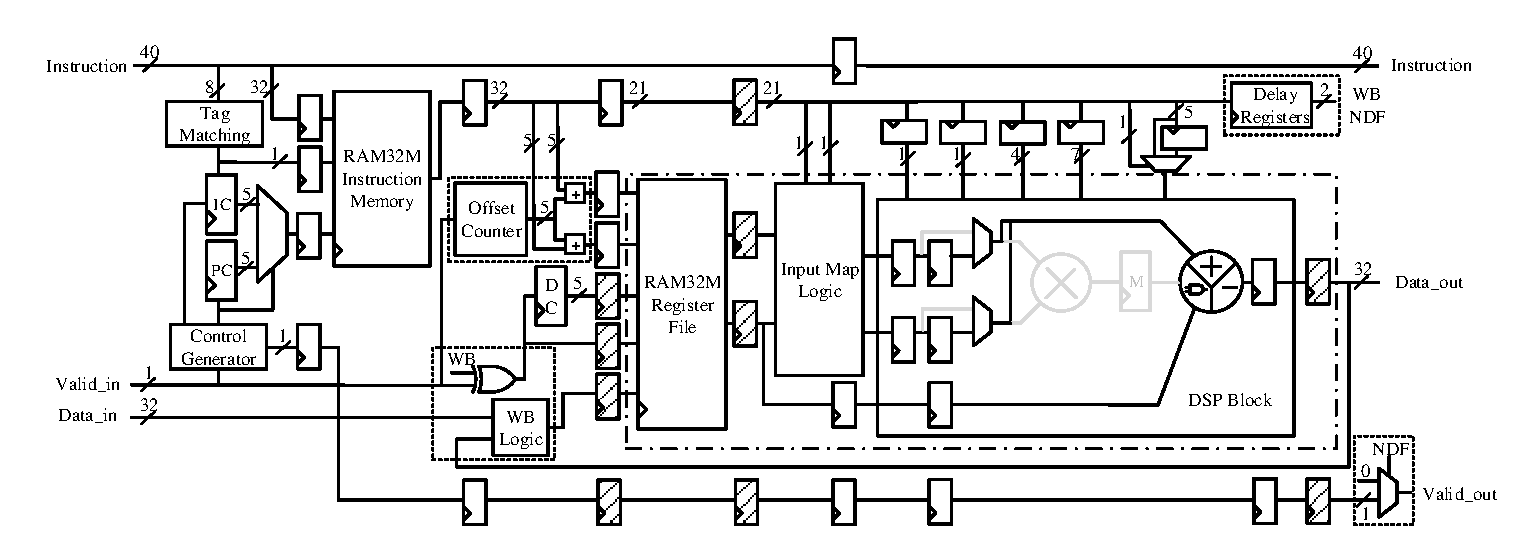
\includegraphics[trim={1cm 0.5cm 1cm 1cm},width=14cm]{figures/FU_WB_new_1.pdf}
	\caption{Proposed time-multiplexed functional unit.}
	\label{fu}
\end{figure*}

\subsection{Architectural Enhancements}
%As discussed earlier, II is one of the critical metrics to determine the throughput of an accelerator for loop kernels.
The II is a critical metric for determining the throughput of an accelerator.
%The II of the overlay in~\cite{li2016area} can be calculated using Equation~\ref{II_V0}. this is significantly higher than that of a spatially configured overlay, and is especially significant for DFGs with a large number of input nodes and operation nodes in the first scheduling stage.
The II of the overlay in~\cite{li2016area} is obtained by the maximum of the number of data load operations plus the number of execution operations with 2 additional clock cycles needed to flush the pipeline among the FUs, as in Equation~\ref{II}.
This is especially large for DFGs with a large number of inputs and operation nodes in the first scheduling stage.
%Equation~\ref{II} gives the II of the overlay in~\cite{li2016area}, which is especially large for DFGs with a large number of inputs and operation nodes in the first scheduling stage. The additional 2 cycles is for flushing the DSP-block pipeline.

\begin{equation}
	II =  \max_{FU} \{\#load + \#op + 2\}
	\label{II}
\end{equation}


\subsubsection{Rotating Register File}
The most obvious way to reduce the II of Equation~\ref{II} is to overlap the loading of input data with instruction execution. 
%Given the simple ASAP operation scheduling shown in~\cite{li2016area}, there is great potential to reduce the II by overlapping the data feeding of RF and the computation of ALU from successive iterations.
Instead of adding additional complexity into the FU to support double-buffering, a rotating register file~\cite{rau1992register} is used to support the overlap of data written into the RF with subsequent instruction execution.
The original design of~\cite{li2016area} used a RAM32M primitive with a dual port configuration (1 read, 1 read/write), whereas the rotating RF version requires a quad port configuration to support 2 reads and 1 write.
The new FU, shown in Fig.~\ref{fu}, includes the offset counter but not the four shaded registers to the left of the RAM32M RF block or the two shaded registers to the right of the DSP block. This design requires 1 DSP block, 196 LUTs, 237 FFs and has a frequency of 334 MHz on a Zynq XC7Z020 (610 MHz on a Virtex-7 VC707).  
%%%The rotating register file allows a new set of input data to be written into later successive locations, which avoids overwriting the current data set.
%Compared with the FU prototype, only an offset counter is added to update the index of read address to avoid the overwritten of successive data set, shown as the left dashed box in Fig.\ref{fu}. 
We refer to this new design as version 1 (V1), and the II is determined as: 
%An example schedule of Fig. 1(b) is given in Section~\ref{ch4_tool} to show the benefit of V1.

\begin{equation}
	II_{V1} =  \max_{FU} \{\#load + 1, \#op + 2\}
	\label{II_V1}
\end{equation}

\noindent where the extra cycle in data load is to separate data blocks.

\subsubsection{Replicating the Stream Datapath}
The II can be reduced, at the expense of an increased data bandwidth requirement, by increasing parallelism.
Replicating the data processing part of the FU (shown within the right dash-dot box) and increasing the data I/O to 64 bits doubles data throughput (halving the II).
This design which reuses the instruction memory and other control circuitry of V1 is called version 2 (V2). It requires 2 DSP blocks, 292 LUTs and 333 FFs, operates at a frequency of 335 MHz and has an II half that of Equation~\ref{II_V1}.

The resource consumption and maximum frequency for the various FU designs on a Zynq XC7Z020 are listed in Table~\ref{FU_table}.
The V1 FU consumes around 22\% more LUTs than that of~\cite{li2016area}, mainly due to the addition of the RAM32M primitive and the offset counter. 
%However, there is an improvement in frequency and a reduction in the number of FFs due to the removal of the registers before the RF.
The resource consumption of V2 is less than twice that of V1, with a similar frequency to V1.

%\begin{equation}
%	II = \{\max_{FU} \{\#load + 1, \#op + 2\}\}/2
%	\label{II_V2}
%\end{equation}


\begin{table}[tb]
	\caption{Comparison of different FU designs.}
	\label{FU_table}
	\centering
	\small
%	\footnotesize
	\begin{tabular}{ccccccc}
		\toprule
		     & ~\cite{li2016area} & V1  & V2  & V3  & V4  & V5  \\ \midrule
		DSPs &         1          &  1  &  2  &  1  &  1  &  1  \\
		LUTs &        160         & 196 & 292 & 212 & 207 & 248 \\
		FFs  &        293         & 237 & 333 & 228 & 163 & 126 \\
		Fmax &        325         & 334 & 335 & 323 & 254 & 182 \\
		IWP  &         --         & --  & --  &  5  &  4  &  3  \\ \bottomrule
	\end{tabular}
\end{table}


%\subsection{Applicability-oriented Architectural Exploration}
%While the performance of the overlay can be improved significantly by reducing the II, it %has to tune to different No. of FUs to fit the DFGs with different depth. 
%A fixed architecture which is able to handle more general applications can be beneficial %to the design productivity, as it save the time for the synthesize of a set of overlay %instances with different requirement of FUs.

\subsubsection{FU Write-back}
The main disadvantage with these overlays is that they are feed-forward only, and thus the overlay depth (and the number of FUs) depends on the critical path of the DFG. 
If output data is written back to the RF, multiple nodes on the DFG critical path could be combined within the same scheduling stage, thus reducing the overlay depth.
%Allowing the output data to be written back to the RF will mean that multiple nodes on the DFG critical path can be combined within the same scheduling stage, thus reducing the overlay depth.
Without write-back, when the application kernel changes the overlay also needs to change, requiring overlay reconfiguration between kernels which significantly impacts the hardware context switch time. 
Thus, a fixed architecture which is able to handle a range of more general kernels would improve execution time when multiple kernels need to be accelerated.

Introducing data write-back is relatively simple and involves feeding the \textit{Data\_out} signal back into the FU and multiplexing it with the \textit{Data\_in} signal, as shown in the lower left dashed box in Fig.~\ref{fu}. 
This requires that the instruction format of~\cite{li2016area} be modified with two extra bits added, a write-back (\textit{WB}) bit and a no data forward (\textit{NDF}) bit. 
Both bits are needed as there is a possibility that the output data will be written back to the RF and bypassed to the next FU stage. Rather than adding two extra bits to the (already) 32-bit instruction, we note that the DSP primitive is only used to support operations with 2 or 3 operands (which means the D port is unused and can be disabled). This means that three bits of the DSP \textit{inmode} field can be hardwired, allowing the use of 1-bit as the \textit{WB} flag, 1-bit as the \textit{NDF} flag, with 1-bit reserved for future use.
The \textit{Valid\_in} signal and the delayed \textit{WB} flag are then used to select between the two different data sources in the write-back logic.

Table~\ref{FU_table} shows the resource utilization, operating frequency and internal write-back path (IWP) for three different implementations of the FU with write-back, referred to as V3, V4 and V5.
The V3 FU is identical to V1, except that the write-back logic is added. That is, it includes all circuitry in Fig.~\ref{fu} apart from the left and right shaded registers.
The IWP is five, comprising one cycle in the RF, one at the register between the RF and the input map logic, and three in the DSP block. This overlay operates at a frequency close to that of the non-WB overlays. 
To reduce the IWP, the registers between the RF RAM32M primitive and the input map logic can be deleted, resulting in a slight frequency reduction. 
This FU, referred to as V4, is identical to V3 except that all shaded registers in Fig.~\ref{fu} are removed. It has an IWP of 4 and a frequency of 254MHz. A further reduction in the IWP can be achieved by reducing the pipeline depth of the DSP block from three to two, resulting in an IWP of 3 and a frequency of 182MHz.

The V3-V5 FUs can then be implemented as a fixed depth overlay, as in Fig.~\ref{pipelines}. We propose implementing two depth 8 overlays in a single tile, with replicated tiles connected via a lightweight NOC, such as in~\cite{kapre2015hoplite}. The two overlays in a tile could either be connected in series (to form a single depth 16 overlay) or connected in parallel to produce a depth 8 overlay with dual datapaths, similar to the V2 based overlay. 

As data forwarding within a DSP block is not possible, due to the inability to access internal signals, it is important to understand the impact of a fixed depth overlay when write-back is used. 
When scheduling DFG nodes to the overlay, any dependency between nodes will require the insertion of NOPs, equal to the IWP, unless other non-dependant nodes can be scheduled between the nodes with the dependency.


\begin{comment}
** need to look at this**
The time-multiplexed FU should adapt its logic with the write-back support for the output data, to fit the operation nodes with data dependency into one scheduling stage. 
A write-back flag with specific delay registers, should be added into the instruction set, which acts as a hint for the output data that need to be restored into the RF for further operations.
An XOR gate is added for the valid signal and the delayed write-back flag to generate the write enable signal for the RF. 
The valid signal and the delayed write-back flag are acting as the select wires for the two different data sources. 
Besides, the scheduling of the load/store data operation and the instruction execution should be very carefully designed, to avoid conflict between the data coming from the previous FU and the feedback data.


%\subsubsection{Adapting the Instruction Set}
%A detailed description of the 32-bit instruction set is shown in Table~\ref{instruction}. 
%It is comprised of four sections, the 19-bit DSP block configuration, the 2-bit input map multiplexing, two 5-bit source operand addresses, and the last bit is reserved for further exploration.
%Since we only use the DSP48E1 primitive to support operations with 2-3 operands (which means D port is disabled), 3 bits ([26:24]) of the inmode can be hardwired as they keep unchanged for the supported operations. 
%Thus, we use 1-bit as the write-back flag and keep the rest 2 bits reserved for further purpose.

\begin{table}[!t]
	\renewcommand{\arraystretch}{1.2}
	\caption{Instruction Format}
	\label{instruction}
	\tiny
	%	\scriptsize
	\centering
	\begin{tabular}{|c|c|c|c|c|c|c|c|}
		\hline
		            &         \multicolumn{4}{c|}{ALU Control}         & \multicolumn{1}{c|}{Input Map} & \multicolumn{2}{c|}{RF Address} \\ \hline
		  Signals   & alumode & inmode  & opmode  & internal registers &           MUX select           & src-1  &         src-2          \\ \hline
		No. of bits &    4    &    5    &    7    &         3          &               2                &   5    &           5            \\ \hline
		 Locations  & [31:28] & [27:23] & [22:16] &      [15:13]       &            [12:11]             & [10:6] &         [5:1]          \\ \hline
	\end{tabular}
\end{table}


By adding the write-back support and a new instruction set, our overlay design (referred as V4) with a fixed No. of FUs is much more flexible to map the feed-forward DFGs with any graph depth. 
However, it inevitably increases the II as this working mechanism may introduce conflict between the feedback of output dada and the data flow coming from the previous FU.
Therefore, we carefully re-examine the FU design to reduce the internal pipeline stages between the input of the RF and the output of the DSP block as much as possible.
Since the RF is implemented by the clocked RAM32M primitive, the registers for the write enable signal, write address and the input data are not necessary. 
Similarly, the registers for the output of DSP block and the valid signal for it can be removed. 
The registers between the RAM32M primitive and the input map logic can be further deleted to trade off 1 less internal pipeline stage, at the cost of slightly frequency degradation. 
As the the registers with shade pattern are removed, the internal computation path is reduced from 6 to 4 clock cycles, and the overall latency of an FU is reduced by 3 clock cycles. 
This new FU design is comprised of 1 DSP block, 207 LUTs and 163 FFs, and it achieves a frequency of 254MHz on the Zynq device. 
\end{comment}
%!TEX root=../draft.tex
%\vspace{-6pt}
\section{Compiling to the Overlay}
\label{ch4_tool}
There are two separate design processes for mapping an application to an overlay. The first is the overlay implementation which is carried out offline using the conventional FPGA design flow. 
At power-on, the bitstream (consisting of the overlay, memory and communication interfaces, and any other components) is used to configure the FPGA.
The second involves mapping the application kernel to the overlay.
To allow for fast vendor independent mapping to the overlay we developed our own mapping tool flow.
This involves, DFG extraction from high-level compute kernels, scheduling the DFG nodes onto the overlay, and finally, instruction generation for each FU. This is typically done offline, however it could also be performed as part of a just-in-time mapping strategy.
On Zynq, the ARM processor loads the kernel configuration into the overlay pipeline and initiates kernel execution.
Our mapping flow is described below using the previous example.

\textbf{\textit{Kernel Mapping:}} The open source HercuLeS HLS tool~\cite{kavvadias2013hardware} is used to transform a `C' description of the compute kernel to a DFG description, where nodes represent operations and edges represent data flow between operations, as shown in Fig.~\ref{dfg}.
For the V1 and V2 based overlays, ASAP scheduling is used which results in no data dependencies between operations at the same scheduling stage, as in~\cite{li2016area}, with nodes in each scheduling stage then being allocated to a single V1 or V2 FU for execution. 
The set of instructions from the sequenced DFG is identified, then the cycle-by-cycle execution pattern is formed which interleaves load/store and arithmetic/ALU operations, as shown in Table~\ref{schedule}. 
For the `gradient' benchmark, the II is reduced from 11 (in~\cite{li2016area}) to 6 (V1) or 3 (V2) with the same ASAP scheduling.
This translates to a throughput of 0.59 Giga-operations/s (GOPS) for the V1 based overlay with a latency of 86.8 ns (1.11 GOPS and 92.4 ns for V2). 
Lastly the 32-bit FU instructions are generated.

\begin{comment}
An overlay has two separate design processes: Overlay implementation on the FPGA and application mapping to the overlay.
While the design and implementation of the overlay relies on the conventional hardware design flow using vendor tools, this process is done offline, once only, and so does not impact the compute kernel implementation of an application. 
We then use an in-house automated compilation flow to provide a rapid, vendor independent, mapping to the overlay.
The mapping process comprises DFG extraction from high-level compute kernels, scheduling of the DFG nodes onto the overlay, and finally, the instruction generation for each FU. This is also done offline.
Then at power-on the bitstream for the overlay, and any other unrelated hardware components, is used to configure the FPGA. Subsequent to this, the ARM processor loads the kernel configuration into the overlay pipeline and initiates kernel execution.
Our mapping flow is described below using the previous example.


\textbf{\textit{HLL to DFG Conversion:}} The tool transforms a `C' description of the compute kernel to a DFG text description, where nodes represent operations and edges represent data flow between operations, as shown in Fig. 1(b).


\textbf{\textit{Operation Scheduling:}} Scheduling is used to generate a sequenced DFG, with nodes in each scheduling stage being allocated to a single FU for execution. 
Here, the set of instructions from the sequenced DFG is identified, then the cycle-by-cycle execution pattern is formed as shown in Table~\ref{schedule}, and lastly the 32-bit FU instructions are generated.
\end{comment}


\begin{table}[b]
	\renewcommand{\arraystretch}{1}
	\caption{First 32 cycles of the `gradient' schedule (II=6).}
	\label{schedule}
	\centering
	\scriptsize
	\resizebox{\columnwidth}{!}{
		\begin{tabular}{lllllllll}
			\toprule
			cycle & \multicolumn{2}{c}{FU0} & \multicolumn{2}{c}{FU1} & \multicolumn{2}{c}{FU2} & \multicolumn{2}{c}{FU4} \\ \midrule
			1     & Load R0 &               &         &               &         &               &         &  \\
			2     & Load R1 &               &         &               &         &               &         &  \\
			3     & Load R2 &               &         &               &         &               &         &  \\
			4     & Load R3 &               &         &               &         &               &         &  \\
			5     & Load R4 &               &         &               &         &               &         &  \\
			6     &         & SUB (R0 R2)   &         &               &         &               &         &  \\
			7     & Load R0 & SUB (R1 R2)   &         &               &         &               &         &  \\
			8     & Load R1 & SUB (R2 R3)   &         &               &         &               &         &  \\
			9     & Load R2 & SUB (R2 R4)   & Load R0 &               &         &               &         &  \\
			10    & Load R3 &               & Load R1 &               &         &               &         &  \\
			11    & Load R4 &               & Load R2 &               &         &               &         &  \\
			12    &         & SUB (R0 R2)   & Load R3 &               &         &               &         &  \\
			13    & Load R0 & SUB (R1 R2)   &         & SQR (R0 R0)   &         &               &         &  \\
			14    & Load R1 & SUB (R2 R3)   &         & SQR (R1 R1)   &         &               &         &  \\
			15    & Load R2 & SUB (R2 R4)   & Load R0 & SQR (R2 R2)   &         &               &         &  \\
			16    & Load R3 &               & Load R1 & SQR (R3 R3)   & Load R0 &               &         &  \\
			17    & Load R4 &               & Load R2 &               & Load R1 &               &         &  \\
			18    &         & SUB (R0 R2)   & Load R3 &               & Load R2 &               &         &  \\
			19    & Load R0 & SUB (R1 R2)   &         & SQR (R0 R0)   & Load R3 &               &         &  \\
			20    & Load R1 & SUB (R2 R3)   &         & SQR (R1 R1)   &         & ADD (R0 R1)   &         &  \\
			21    & Load R2 & SUB (R2 R4)   & Load R0 & SQR (R2 R2)   &         & ADD (R2 R3)   &         &  \\
			22    & Load R3 &               & Load R1 & SQR (R3 R3)   & Load R0 &               &         &  \\
			23    & Load R4 &               & Load R2 &               & Load R1 &               & Load R0 &  \\
			24    &         & SUB (R0 R2)   & Load R3 &               & Load R2 &               & Load R1 &  \\
			25    & Load R0 & SUB (R1 R2)   &         & SQR (R0 R0)   & Load R3 &               &         & ADD (R0 R1)   \\
			26    & Load R1 & SUB (R2 R3)   &         & SQR (R1 R1)   &         & ADD (R0 R1)   &         &  \\
			27    & Load R2 & SUB (R2 R4)   & Load R0 & SQR (R2 R2)   &         & ADD (R2 R3)   &         &  \\
			28    & Load R3 &               & Load R1 & SQR (R3 R3)   & Load R0 &               &         &  \\
			29    & Load R4 &               & Load R2 &               & Load R1 &               & Load R0 &  \\
			30    &         & SUB (R0 R2)   & Load R3 &               & Load R2 &               & Load R1 &  \\
			31    & Load R0 & SUB (R1 R2)   &         & SQR (R0 R0)   & Load R3 &               &         & ADD (R0 R1)   \\
			32    & Load R1 & SUB (R2 R3)   &         & SQR (R1 R1)   &         & ADD (R0 R1)   &         &  \\ \bottomrule
		\end{tabular}
	}
\end{table}

Typically, most of the existing CGRA architectures adopt Modulo scheduling~\cite{rau1994iterative}, or a derivative algorithm, to achieve a minimum II. 
However, Modulo scheduling is based on the assumption that each operation node is executed in 1 cycle and the transfer of data between two arbitrary FUs completes in 1 cycle, which is not realistic for highly pipelined architectures. 
Instead, for a fixed depth overlay we use an iterative greedy scheduling strategy which groups DFG nodes at each scheduling step into clusters and then adds DFG nodes along the critical path from subsequent clusters, while balancing the II across all clusters.
The number of scheduling clusters is equal to the overlay depth.
Due to space constraints, the scheduling algorithm will not be discussed further.
%, which in this case is 8.

As an example of fixed depth overlay scheduling, consider the `qspline' benchmark, of Fig.~\ref{qspline}. Here, the critical path is 8 and we map to a depth 4 overlay (4 FUs). Scheduling produces the 4 instruction clusters shown in Fig.~\ref{qspline} (using red dashes). NOPs (equal to IWP-1) must be added between dependant instructions (DFG nodes) unless other non-dependant instructions can be scheduled in between. For example, in the first (top) cluster, Node 17 is scheduled, followed by 13, 25, 9, 20, and 12, before 15 is scheduled. Hence, the dependency between 17 and 15 is resolved and no NOPs are inserted. 
Similarly for the 2nd cluster, scheduling as: 14, 26, 21, 10, 16, 11, 27, 22, resolves dependencies 14-11, 26-27, and 21-22, for all overlay versions. In cluster three, scheduling as: 18, 24, 28, 23, 19, 30, 8, resolves all dependencies for the V4 and V5 overlays, but not for the V3 overlay, which with an IWP of 5 requires 4 operations between dependant nodes. Hence, a single NOP must be added between 23 and 19 which then resolves all 4 sets of dependant instructions.
For the 4th cluster, graph balancing is performed, and the two additions scheduled, followed by IWP-1 NOPs before the final addition.
%(equal to IWP-1) must be added between 31 and 32, and 32 and 29. 

%Here the V3 overlay has an II of 17, with a throughput of 0.45 Giga-operations/s (GOPS) and the latency of 135ns, while the V4 overlay has 14, 0.43 GOPS and 151ns, respectively (compared to the depth 8 V1 overlay with 11, 0.69 GOPS and 234ns, respectively). 

The consequences of a fixed depth overlay are an increase in the II with a corresponding reduction in the throughput, but with a significant reduction in the latency. For the `qspline' benchmark, the V3 overlay has an II of 15, with a throughput of 0.51 GOPS and a latency of 125 ns, while the V4 overlay has an II of 14, a throughput of 0.43 GOPS and a latency of 148 ns. This compares to the depth 8 V1 overlay with an II of 11, a throughput of 0.69 GOPS and a latency of 234ns. 
%It should be noted, that in some cases, limiting the depth of the overlay and properly balancing the schedule between stages actually results in a reduction in the II, compared to the simple ASAP schedule used in the V1 overlay, as can be seen in Table~\ref{benchmarks}. 



\begin{comment}
Therefore, this paper is focusing on architectural exploration, and an ASAP scheduling is generated for the `gradient' benchmark shown as indicated in Table~\ref{schedule}, which takes advantage of the rotating register file. 
It is applicable to the design of V1 and V2 as there is no data dependency between operations at the same stage.
Similar to the operation scheduling for~\cite{li2016area}, input data coming from the FIFO channel are loaded into the RF of FU0 at the initial 5 cycles (from clock cycle 1 to clock cycle 5).
As soon as loading has completed, FU0 is triggered at the 6th clock cycle and starts executing the 4 SUB instructions using the data from the RF, with a cycle-by-cycle fashion. 
FU0 starts sending the resulting data to FU1 on the 9th clock cycle (due to the 3 stage internal pipeline in the DSP block) and then waits for the cycle to repeat. 
The operations of FU1, FU2 and FU3 are similar to that of FU0, and the result of FU3 is sent back to the output FIFO channel on the 28th clock cycle.
The only difference between the scheduling of V1/V2 and~\cite{li2016area} is that, each FU is able to fetch another set of data from the previous stage without waiting for all the operations to be finished. 
Regarding to the load/store and arithmetic/ALU operations belong to each FU respectively, we find that the maximum value generated from Equation~\ref{II_V1} is 6 for this particular benchmark. 
That means, the II is reduced from 11 (\cite{li2016area}) to 6 (V1) with the same ASAP scheduling.
Similarly, the II of V2 can be further reduced to 3. 


Noted that this simple scheduling may cause conflict on V4 when the data from previous stage and the feedback data are writing to the RF at the same time, the computing operations should be triggered as soon as the necessary data are valid in the RF. 
The order of the instructions also needs to tune to make sure that the feedback data are ready before the execution of associated instructions to avoid NOP insertions.
The `qspline' benchmark is indicated as an example to show the scheduling of V4, shown in Fig.~\ref{qspline}. 
The operation nodes marked as N12, N20, N9, N25, N13, N17 and N15 are clustering into the first schedule stage. 
The second stage consists of operation nodes N10, N21, N26, N14, N27, N11 and N16, while N28, N22, N24, N18, N8, N23, N30 and N19 are grouped into the third stage. 
The last three operation nodes N31, N32 and N29 are scheduled in the final stage. 
In this scheduling, we achieve a significant reduction of the No. of FU from 8 to 4 compared to V1, with a modest penalty of II increase from 11 to 15.
\end{comment}

\begin{figure}[tb]
	\centering
	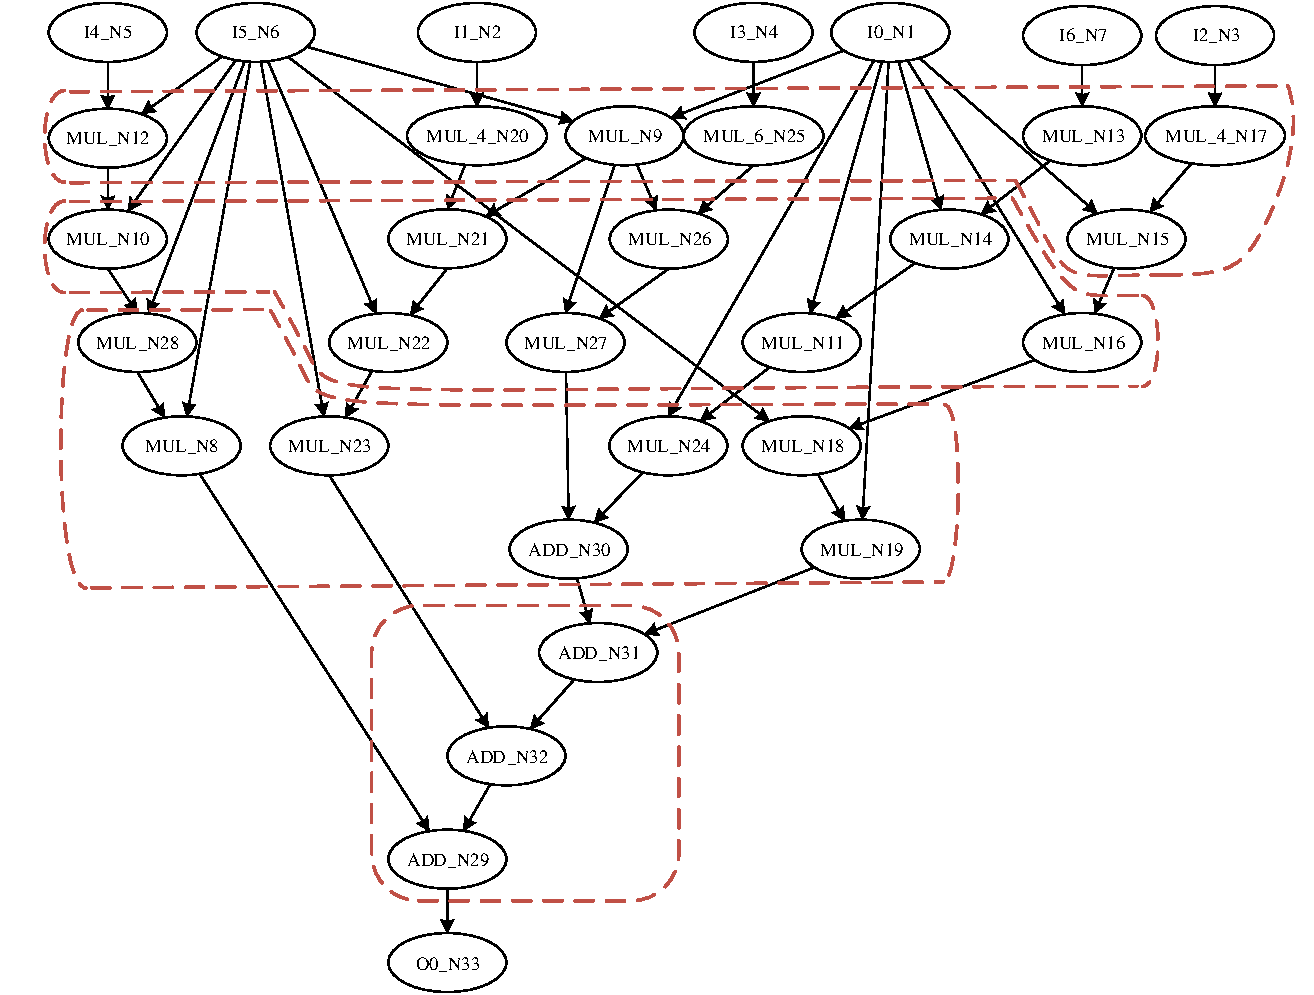
\includegraphics[width=8cm]{figures/Cluster_qspline.pdf}
	\caption{Data flow graph of the `qspline' benchmark.}
	\label{qspline}
\end{figure}



%Section End
%!TEX root=../draft.tex
\section{Experimental Evaluation}
\label{ch5_experiments}

We compare the performance of our linear TM overlays using a set of compute kernels from~\cite{jain2015efficient,binipolynomial}, as shown in Table~\ref{benchmarks}.
The V1 (1 DSP, no WB), V2 (2 DSP, no WB), V3 (WB, IWP=5) and V4 (WB, IWP=4) overlays are compared to the overlay in~\cite{li2016area}. 
V1, V2 and the overlay in~\cite{li2016area} have a depth equal to the critical path, and are configured on a kernel by kernel basis, while V3 and V4 have a fixed depth of eight. 
All overlays are implemented on a Zynq XC7Z020.

The FPGA DSP and logic slice utilization, and operating frequency, for different depth V1 and V2 overlays are shown in Fig.~\ref{scalability} (V3 and V4 are not included in this figure as they have a fixed depth). A depth 8 V1 overlay consumes 654 logic slices and 8 DSP slices which represents less than 5\% of the logic and DSP resources on Zynq. The depth 8 V2 overlay consumes 893 logic slices and 16 DSP blocks or less than 8\% of the Zynq resources. 
By comparison, the fixed depth (of 8) V3 (and V4) overlay consumes 814 (817) logic slices, 8 (8) DSP slices and operates at a frequency of 286MHz (233MHz).

The DFG characteristics (number of I/O, number of arithmetic operations and graph depth) for the chosen benchmarks and the II achieved when mapped to the various overlays are shown in Table~\ref{benchmarks}. For the first three benchmarks, which have a depth $\leq$ 8, ASAP scheduling is used to map to the V3 and V4 overlays, and thus, the II is the same as for the V1 overlay. 
The V1 (V2) overlay has an average 42\% (71\%) reduction in the II, compared to~\cite{li2016area}.
The V3 (V4) overlay has an average 34\% (40\%) reduction in the II for the depth $>$ 8 benchmarks.
%with depth $>$ 8, compared to~\cite{li2016area}.

\begin{comment}
Among the feed-forward only overlays such as~\cite{li2016area}, V1, and V2, their requirement for the number of FUs is determined by the graph depth of each benchmark. 
The II is high for benchmarks with a large number of I/O nodes and high parallelism, where parallelism stands for the average number of operations per schedule stage.
It can be used to roughly measure the throughput, as all the three overlays run at a frequency with a slight degradation from around 330MHz to 300MHz on Zynq XC7Z020, as shown in Fig.~\ref{fmax}. 
According to Table~\ref{benchmarks} and Fig.~\ref{resources}, V1 generally reduces the II into half with almost the same resource consumption as~\cite{li2016area}, and V2 further achieves down to a quarter with an incremental area overhead.
As there are no loop carried dependencies, we can replicate multiple streaming models as in Fig.~\ref{pipelines} to reduce the II into a theoretical minimum of 1.
\end{comment}

\begin{table}[t]
	\renewcommand{\arraystretch}{1}
	\caption{DFG characteristics of benchmark set.}
	
	\label{benchmarks}
	\centering
%	\scriptsize 
	\resizebox{\columnwidth}{!}{
		\begin{tabular}{cccccccccc}
			\toprule
			No. & Benchmark & I/O & \#Ops & Depth & II$_{\cite{li2016area}}$ & II$_{V1}$ & II$_{V2}$ & II$_{V3}$ & II$_{V4}$ \\ \midrule
			1.  & chebyshev & 1/1 &   7   &   7   &            6             &     4     &     2     &     4     &     4     \\
			2.  &  mibench  & 3/1 &  13   &   6   &            14            &     8     &     4     &     8     &     8     \\
			3.  &  qspline  & 7/1 &  25   &   8   &            19            &    11     &    5.5    &    11     &    11     \\
			4.  & sgfilter  & 2/1 &  18   &   9   &            13            &     8     &     4     &     8     &     8     \\
			5.  &   poly5   & 3/1 &  27   &   9   &            19            &    11     &    5.5    &    11     &    11     \\
			6.  &   poly6   & 3/1 &  44   &  11   &            25            &    14     &     7     &    13     &    12     \\
			7.  &   poly7   & 3/1 &  39   &  13   &            24            &    14     &     7     &    20     &    17     \\
			8.  &   poly8   & 3/1 &  32   &  11   &            21            &    12     &     6     &    16     &    14     \\ \bottomrule
		\end{tabular}
	}
	
\end{table}

%\pgfdeclarelayer{background}
%\pgfdeclarelayer{foreground}
%\pgfsetlayers{background,main,foreground}

\pgfplotsset{
	axis background/.style={fill=none},
	%tick style=mygrey2,
	%tick label style=mygrey2,
	grid=none,
	%xtick pos=left,
	%ytick pos=left,
	tick style={
		major grid style={style=white,line width=1pt},minor grid style=white,
%		major grid style={style=white,line width=1pt},minor grid style=mygrey3,
		%tick align=outside,
	},
	%minor tick num=4,
}

\begin{figure}[b]
	\centering
	\begin{subfigure}[]{0.23\textwidth}
		\centering	
		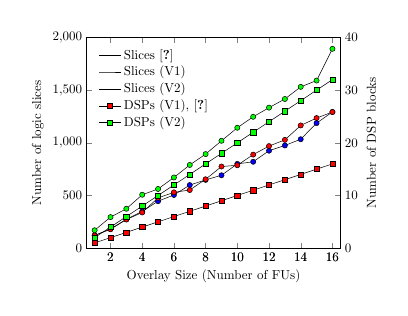
\begin{tikzpicture}[scale = 0.47]
		\begin{axis}[
%		xlabel=Overlay Size (Number of FUs),
		ylabel=Number of logic slices,
		ymax = 2000,
		%ymax = 2500,
		ymin = 0,
		xmax = 16.5,
	    xmin = 0.5,
		legend pos=north west,
		legend cell align={left},
		legend style={draw=none}
		]    
		
		\addplot [mark=*,mark options={fill=blue}] plot coordinates {
			(1,     121)
			(2,     183)
			(3,     274)
			(4,     349)
			(5,     446)
			(6,     505)
			(7,     599)
			(8,     648)
			(9,     692)
			(10,    800)
			(11,    820)
			(12,    925)
			(13,    975)
			(14,    1034)
			(15,    1187)
			(16,    1293)									
		};
		\label{S_olaf}
		\addlegendentry{Slices~\cite{li2016area}}
		
		\addplot [mark=*,mark options={fill=red}] plot coordinates {
			(1,     121)
			(2,     179)
			(3,     272)
			(4,     339)
			(5,     477)
			(6,     530)
			(7,     552)
			(8,     654)
			(9,     775)
			(10,    787)
			(11,    888)
			(12,    969)
			(13,    1028)
			(14,    1165)
			(15,    1235)
			(16,    1292)									
		};
		\label{S_V1}
		\addlegendentry{Slices (V1)}
	
		\addplot [mark=*,mark options={fill=green}] plot coordinates {
			(1,     170)
			(2,     295)
			(3,     374)
			(4,     507)
			(5,     562)
			(6,     671)
			(7,     790)
			(8,     893)
			(9,     1019)
			(10,    1143)
			(11,    1247)
			(12,    1334)
			(13,    1416)
			(14,    1531)
			(15,    1591)
			(16,    1892)			
		};
		\label{S_V2}
		\addlegendentry{Slices (V2)} 
%		\legend{Slices~\cite{li2016area}\\Slices (V1)\\Slices (V2)\\}     
		\end{axis}
		
		\begin{axis}[
		axis y line*=right,
		xlabel=Overlay Size (Number of FUs),
		ylabel=Number of DSP blocks,
		ymax = 40,
		%ymax = 50,
		ymin = 0,
		xmax = 16.5,
	    xmin = 0.5,
		legend pos=north west,
		legend cell align={left},
		legend style={draw=none}
		]
		\addlegendimage{/pgfplots/refstyle=S_olaf}\addlegendentry{Slices~\cite{li2016area}}
		\addlegendimage{/pgfplots/refstyle=S_V1}\addlegendentry{Slices (V1)}
		\addlegendimage{/pgfplots/refstyle=S_V2}\addlegendentry{Slices (V2)}

		\addplot [mark=square*,mark options={fill=red}] plot coordinates {
			(1,     1)
			(2,     2)
			(3,     3)
			(4,     4)
			(5,     5)
			(6,     6)
			(7,     7)
			(8,     8)
			(9,     9)
			(10,    10)
			(11,    11)
			(12,    12)
			(13,    13)
			(14,    14)
			(15,    15)
			(16,    16)		
		};
		\addlegendentry{DSPs (V1),~\cite{li2016area}} 
		
		\addplot [mark=square*,mark options={fill=green}] plot coordinates {
			(1,     2)
			(2,     4)
			(3,     6)
			(4,     8)
			(5,     10)
			(6,     12)
			(7,     14)
			(8,     16)
			(9,     18)
			(10,    20)
			(11,    22)
			(12,    24)
			(13,    26)
			(14,    28)
			(15,    30)
			(16,    32)				
		};
		\addlegendentry{DSPs (V2)}
				
%		\legend{DSPs (V1),~\cite{li2016area}\\DSPs (V2)\\}	
		\end{axis}
		\end{tikzpicture}		
		\caption{Resource Usage}
		\label{resources}
		
	\end{subfigure}
	~
%	\hfill
%	\\
	\begin{subfigure}[]{0.23\textwidth}
		\centering	
	 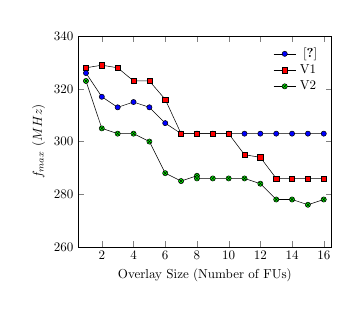
\begin{tikzpicture}[scale = 0.47]
	 \begin{axis}[
	 xlabel=Overlay Size (Number of FUs),
	 ymin=260,
	 ymax=340,
	 %ymin=200,
	 %ymax=400,
	 xmax = 16.5,
	 xmin = 0.5,
	 ylabel=$f_{max}$ ($MHz$),
	 legend pos=north east,
	 legend style={draw=none}
	 ]    

	\addplot [mark=*,mark options={fill=blue}] plot coordinates {
		(1,     326)
		(2,     317)
		(3,     313)
		(4,     315)
		(5,     313)
		(6,     307)
		(7,     303)
		(8,     303)
		(9,     303)
		(10,    303)
		(11,    303)
		(12,    303)
		(13,    303)
		(14,    303)
		(15,    303)
		(16,    303)	
	}; 
	 \addplot [mark=square*,mark options={fill=red}] plot coordinates {
	 	(1,     328)
	 	(2,     329)
	 	(3,     328)
	 	(4,     323)
	 	(5,     323)
	 	(6,     316)
	 	(7,     303)
	 	(8,     303)
	 	(8,     303)
	 	(9,     303)
	 	(10,    303)
	 	(11,    295)
	 	(12,    294)
	 	(13,    286)
	 	(14,    286)
	 	(15,    286)
	 	(16,    286)
	 }; 
	 \addplot [mark=otimes*,mark options={fill=green}] plot coordinates {
	 	(1,     323)
	 	(2,     305)
	 	(3,     303)
	 	(4,     303)
	 	(5,     300)
	 	(6,     288)
	 	(7,     285)
	 	(8,     287)
	 	(8,     286)
	 	(9,     286)
	 	(10,    286)
	 	(11,    286)
	 	(12,    284)
	 	(13,    278)
	 	(14,    278)
	 	(15,    276)
	 	(16,    278) 	
	 };

	 \legend{~\cite{li2016area}\\V1\\V2\\}
	 \end{axis}

	 \end{tikzpicture}	
	 \caption{$f_{max}$ Drop}
	 \label{fmax}
	%}
	\end{subfigure}
	
	\caption[]{V1 and V2 overlay scalability on Zynq XC7Z020.} 
	\label{scalability}
	
\end{figure}



Fig.~\ref{throughput_latency} shows the throughput and latency of the different overlays for the benchmarks given in Table~\ref{benchmarks}. 
In terms of throughput, all overlays have a higher throughput than the overlay of~\cite{li2016area}. This is because interleaving data transfer with execution reduces the II and hence improves throughput.
The two DSP V2 overlay has approximately twice the throughput as the V1 overlay, but also requires twice the data bandwidth. The size of both of these overlays is dependant on the depth (critical path) of the application kernel's DFG, and needs to be reconfigured when the application kernel changes.
A depth 8 V1 (V2) overlay requires a minimum reconfigurable region of 7 (9) CLB tiles and 1 (2) DSP tile with a configuration time of 0.73 (1.02) ms using the processor configuration access port (PCAP). Additionally, the overlays require a further 0.29$\mu s$ to load the configuration data for the largest benchmark.

The single DSP V3 overlay has a throughput similar to the V1 overlay, with an average reduction of just 10\%. The V4 overlay has a slightly reduced throughput as it operates at a lower frequency due to the removal of pipeline registers to reduce the IWP.
The V3 and V4 overlays both have a fixed depth (in these experiments a depth of 8 is used).
Adding write-back capabilities allows larger kernels to be mapped to a smaller number of FUs, removing the requirement that the overlay depth must be the same as the kernel critical path. This eliminates the need to reconfigure the overlay when the application kernel changes, making the overlay more general purpose (but requiring a different scheduling strategy).
Thus, a hardware context switch on the V3 overlay requires just 0.25$\mu s$ for the largest benchmark, representing a 2900$\times$ reduction compared to the V1 overlay.

The latency is heavily dependent on the depth of the overlay. For the V1 and V2 overlays and the overlay of~\cite{li2016area}, the overlay depth is equal to the DFG depth, due to the ASAP scheduling strategy used, and hence these overlays all have a larger latency. The V3 and V4 overlays generally show a significant reduction in the latency, particularly for larger depth DFGs, due to the fixed overlay depth. 



\pgfplotsset{
	axis background/.style={fill=white},
	tick style=black,
	tick label style=black,
	grid=both,
	xtick pos=left,
	ytick pos=left,
	tick style={
		major grid style={style=white,line width=1pt},minor grid style=white,
		tick align=outside,
	},
	minor tick num=4,
}

\begin{figure}[tb]
	\centering
	\begin{subfigure}[]{0.5\textwidth}
		\centering
		\pgfplotstableread{
			0		0.35	0.53	1.00	0.50	0.43
			1		0.29	0.50	0.94	0.46	0.38 
			2		0.40	0.69	1.30	0.65	0.53
			3		0.42	0.68	1.29	0.64	0.52
			4		0.43	0.74	1.40	0.70	0.57
			5		0.53	0.93	1.80	0.97	0.85
			6		0.49	0.80	1.55	0.56	0.53 
			7		0.46	0.79	1.53	0.57	0.53
		}\datathroughput
		\begin{tikzpicture}
		\centering
		\begin{axis}[ybar=0pt,
		width=17cm,
		x = 0.85cm,
		height=4.3cm,
		ymin=0,
		ymax=2,        
		ylabel={Throughput (GOPS)},
		grid style={dotted,gray},
		ymajorgrids=true,
		%	nodes near coords,    
		xtick=data,
		bar width = 0.15,
		xticklabels = {
			\strut 1,
			\strut 2,
			\strut 3,
			\strut 4,
			\strut 5,
			\strut 6,
			\strut 7,
			\strut 8                                   
		},
		x tick label style={rotate=45, anchor=north east, inner sep=0mm},
		major x tick style = {opacity=0},
		minor x tick num = 1,
		minor tick length=1ex,
		%	every node near coord/.append style={
		%		anchor=west,
		%		rotate=90,
		%		font=\tiny
		%	},
		]
		
		\addplot[draw=black,fill=blue, draw opacity=1] table[x index=0,y index=1] \datathroughput;\label{T_olaf}
		\addplot[draw=black,fill=red, draw opacity=1] table[x index=0,y index=2]   \datathroughput;\label{T_V1} 
		\addplot[draw=black,fill=green, draw opacity=1] table[x index=0,y index=3] \datathroughput;\label{T_V2} 
		\addplot[draw=black,fill=yellow, draw opacity=1] table[x index=0,y index=4] \datathroughput;\label{T_V3} 
		\addplot[draw=black,fill=cyan, draw opacity=1] table[x index=0,y index=5]  \datathroughput;\label{T_V4} 
		
		\end{axis}
		\node [draw=none, fill=white] at (rel axis cs: 0.55,1.2) {\shortstack[l]{
				\ref{T_olaf}~\cite{li2016area} \ref{T_V1} V1 \ref{T_V2} V2} \ref{T_V3} V3 \ref{T_V4} V4};	
		\end{tikzpicture}
%		\caption{Throughput in GOPS.}
		\label{throughput}
	\end{subfigure}
	
	\begin{subfigure}[]{0.5\textwidth}
		\centering
		\pgfplotstableread{
			0		116	116	123	105	129
			1		143	139	154	105	129
			2		235	235	249	147	181
			3		198	198	210	151	181
			4		248	248	263	165	198
			5		373	385	396	200	224
			6		400	424	436	231	258
			7		320	330	340	203	237
		}\datalatency
		\begin{tikzpicture}
		\centering
		\begin{axis}[ybar=0pt,
		width=17cm,
		x = 0.85cm,
		height=4.3cm,
		ymin=0,
		ymax=500,        
		ylabel={Latency (ns)},
		grid style={dotted,gray},
		ymajorgrids=true,
		%	nodes near coords,    
		xtick=data,
		bar width = 0.15,
		xticklabels = {
			\strut 1,
			\strut 2,
			\strut 3,
			\strut 4,
			\strut 5,
			\strut 6,
			\strut 7,
			\strut 8                                   
		},
		x tick label style={rotate=45, anchor=north east, inner sep=0mm},
		major x tick style = {opacity=0},
		minor x tick num = 1,
		minor tick length=1ex,
		%	every node near coord/.append style={
		%		anchor=west,
		%		rotate=90,
		%		font=\tiny
		%	},
		]
		
		\addplot[draw=black,fill=blue, draw opacity=1] table[x index=0,y index=1] \datalatency;\label{L_olaf}
		\addplot[draw=black,fill=red, draw opacity=1] table[x index=0,y index=2] \datalatency;\label{L_V1} 
		\addplot[draw=black,fill=green, draw opacity=1] table[x index=0,y index=3] \datalatency;\label{L_V2} 
		\addplot[draw=black,fill=yellow, draw opacity=1] table[x index=0,y index=4] \datalatency;\label{L_V3} 
		\addplot[draw=black,fill=cyan, draw opacity=1] table[x index=0,y index=5] \datalatency;\label{L_V4} 
		
		\end{axis}
%		\node [draw=none, fill=white] at (rel axis cs: 0.5,0.85) {\shortstack[l]{
%				\ref{L_olaf}~\cite{li2016area}  \ref{L_V1} V1  \ref{L_V2} V2} \ref{L_V3} V3 \ref{L_V4} V4};	
		\end{tikzpicture}
%		\caption{Latency in ns.}
		\label{latency}
	\end{subfigure}
	
	\caption{Throughput and latency for the benchmarks.}
	\label{throughput_latency}
\end{figure}

\begin{comment}
To demonstrate the benefits of the proposed linear TM overlays, we compare different versions of the linear TM overlays with one of the more efficient spatially configured overlays from the literature~\cite{jain2015efficient}.
For all the implementations we use the minimal number of FUs/hardware for the benchmark implementations, except for V4 with a fix architecture of 8 FUs.
This is to observe the effect of FU reduction on the area requirement, and the benefit of mapping all the benchmarks without overlay reconfiguration.
Fig.~\ref{fu_comparison} shows the number of FUs required for the linear TM overlay V1/V2 compared to that of the spatially configured overlay in~\cite{jain2015efficient} for each of the benchmarks in Table~\ref{benchmarks}. 
There is a significant reduction in the number of FUs required for V1/V2, but at the expense of an increase in the II compared to~\cite{jain2015efficient}. 
The most remarkable advantage of V4 is that it can handle all the benchmarks regardless of the graph depth, which significantly reduce the context switch time for different compute kernels.

%\pgfplotsset{
	axis background/.style={fill=white},
	tick style=black,
	tick label style=black,
	grid=both,
	xtick pos=left,
	ytick pos=left,
	tick style={
		major grid style={style=white,line width=1pt},minor grid style=white,
		tick align=outside,
	},
	minor tick num=4,
}

\begin{figure}[tb]
%\vspace{-18pt}
\centering
%\pgfplotstableread{
%	0  5			7     
%	1  12      		9     
%	2  8	     	6      
%	3  22    		8 
%	4  17    		9      
%	5  30     		11    
%	6  28     		13       
%	7  19      		11
%}\dataset
\pgfplotstableread{
	0  		 5		7     8
	1  		 12     9     8
	2  		 8	    6     8 
	3  		 22    	8 	  8
	4  	 	 17    	9     8
	5  		 30     11    8
	6  		 28     13    8
	7  		 19     11    8
}\dataset
\begin{tikzpicture}
\centering
\begin{axis}[ybar=0pt,
%enlarge x limits=0.05,
width=17cm,
x = 0.85cm,
height=4.3cm,
ymin=0,
ymax=100,        
ylabel={Number of FUs required},
grid style={dotted,gray},
ymajorgrids=true,
nodes near coords,    
xtick=data,
bar width = 0.25,
%xticklabels={1,2,...,26},
xticklabels = {
	\strut 1,
	\strut 2,
	\strut 3,
	\strut 4,
	\strut 5,
	\strut 6,
	\strut 7,
	\strut 8
%	\strut 26 (1)                                    
},
x tick label style={rotate=45, anchor=north east, inner sep=0mm},
major x tick style = {opacity=0},
minor x tick num = 1,
minor tick length=1ex,
every node near coord/.append style={
        anchor=west,
        rotate=90,
        font=\tiny
},
]

\addplot[draw=black,fill=blue!80, draw opacity=1] table[x index=0,y index=1] 
\dataset; \label{scoverlay}
\addplot[draw=black,fill=black!70, draw opacity=1] table[x index=0,y index=2] \dataset;\label{tmoverlay_1} 
\addplot[draw=black,fill=green!60, draw opacity=1] table[x index=0,y index=3] \dataset;\label{tmoverlay_2} 

\end{axis}
	\node [draw=none, fill=white] at (rel axis cs: 0.5,0.72) {\shortstack[l]{
			\ref{scoverlay} Spatially Configured Overlay~\cite{jain2015efficient} \\ \ref{tmoverlay_1} V1/V2 \\ \ref{tmoverlay_2} V4}};

\end{tikzpicture}
\caption{Number of FUs required for the benchmarks.}
\label{fu_comparison}
%\vspace{-9pt}
\end{figure}
\end{comment}

\section{Conclusion}
\label{ch6_conclusion}
We have presented an area efficient FPGA overlay with a linear connection of TM FUs based on the Xilinx DSP48E1.
Interleaving data transfer with instruction execution significantly reduces the II with a resulting increase in throughput.
Introducing write-back into the FU design allows the overlay depth to be fixed. 
%Introducing write-back into the FU design and modifying the scheduling strategy allows the overlay depth to be fixed.
This eliminates the need to reconfigure the overlay if the application kernel changes, making the overlay more general. These changes significantly reduce the latency with just a small decrease in throughput.
The V3 overlay has the best performance, as for a fixed data bandwidth, it has comparable throughput with a significantly reduced latency.





\def\IEEEbibitemsep{1pt plus 1pt}
%\footnotesize
%\scriptsize
\bibliographystyle{abbrv}
%\bibliographystyle{acm}
% argument is your BibTeX string definitions and bibliography database(s)
\bibliography{sigproc,files/references}


% that's all folks
\end{document}


